\documentclass[11pt]{article}
\usepackage[english]{babel}

% Packages
\usepackage{graphicx}
\usepackage{wrapfig}
\usepackage{fullpage}
\usepackage{multirow}
\usepackage{amsmath}
\usepackage{bm}
\usepackage{hyperref}
\usepackage{fancyhdr}
\usepackage{enumitem}
\usepackage{color}
\usepackage{framed}
\usepackage{nicefrac}
\usepackage{units}
\usepackage{amstext}
\usepackage{amsmath} 
\usepackage{amssymb}
\usepackage{cite}
\usepackage{color}
\usepackage[usenames,dvipsnames,svgnames,table]{xcolor}
\usepackage{psfrag}
\usepackage{subfigure}
\usepackage{array}
\usepackage{threeparttable}
\usepackage{dcolumn}
\newcolumntype{d}{D{.}{.}{-1}}
\usepackage{enumitem}
\usepackage{titlesec}
\usepackage{placeins}
\usepackage{soul}
\usepackage{comment}
\usepackage[sort,numbers]{natbib}
% Margins
\setlength{\oddsidemargin}{0pt}
\setlength{\topmargin}{-0.3in}
\setlength{\headheight}{0in}
\setlength{\headsep}{30pt}
\setlength{\topskip}{0pt}
\setlength{\textheight}{8.75in}
\setlength{\textwidth}{6.5in}
\setlength{\hoffset}{0pt}
\setlength{\voffset}{0pt}

% My definitions
\def\bm#1{\mbox{\boldmath{$#1$}}}
\DeclareMathAlphabet{\bbm}{U}{bbm}{m}{sl}
\newcommand\etc{etc.\ }
\newcommand\eg{e.g.\ }
\newcommand\ie{i.e.\ }
\newenvironment{myindentpar}[1]{\begin{list}{}{\setlength{\leftmargin}{0.5in}}\item[#1]}{\end{list}}
\renewcommand{\v}[1]{{\mbox{\boldmath $#1$}}}
\newcommand{\wh}[1]{\widehat{#1}}
\newcommand{\wt}[1]{\widetilde{#1}}
\newcommand{\ol}[1]{\overline{#1}}
\newcommand{\Gv}{\l^2}
\newcommand{\sig}{\widehat{\sigma}}
\newcommand{\ddt}[1]{\frac{\partial #1}{\partial t}}
\newcommand{\We}{\mathrm{We}}
\newcommand{\eps}{\varepsilon}
\newcommand{\tm}{\mathrm}
\usepackage[font={footnotesize}]{caption}

% Some colors
\definecolor{light-gray}{gray}{0.95}

% Colors in titles
\titleformat{\section}
{\color{DarkBlue}\normalfont\Large\bfseries}
{\color{DarkBlue}\thesection}{1em}{}

% Start document
\begin{document}

% First page style
\thispagestyle{fancy}
\fancyhf{}
\renewcommand{\headrulewidth}{0pt}
\lfoot{\textsc{XSEDE \hspace{0.01in}  \textbar \hspace{0.01in}  \textcolor{gray}{Research Allocation Proposal}}}
\rfoot{\textcolor{gray}{\textsc{Page}} \hspace{0.05in} \textbar \hspace{0.01in} \thepage}

% Header and footer %%%%%%%%%%%%%%%%%%%%%%%%%%%%%%%%%%%%%%%%%%
\pagestyle{fancy}
\fancyhf{}
\renewcommand{\headrulewidth}{0pt}
%\lhead{\small{\textsc{Cornell University \hspace{0.01in}  \textbar \hspace{0.01in} Desjardins}}}
%\rhead{\small{\textsc{Multiphase flows with AMR}}}
\lfoot{\textsc{XSEDE \hspace{0.01in}  \textbar \hspace{0.01in}  \textcolor{gray}{Research Allocation Proposal}}}
\rfoot{\textcolor{gray}{\textsc{Page}} \hspace{0.05in} \textbar \hspace{0.01in} \thepage}
%%%%%%%%%%%%%%%%%%%%%%%%%%%%%%%%%%%%%%%%%%%%%%%%%%%%%

\newcommand{\fc}[1]{\textcolor{blue}{#1}}


\graphicspath{{./Images/}}

% START INTRODUCTION %%%%%%%%%%%%%%%%%
\begin{center} \textbf{ \color{DarkBlue} \LARGE{AMReX Multiphase Flow Solver}} \\
%\vspace{0.08in}
%\textbf{\color{DarkBlue} \LARGE{Turbulent Atomizing Liquid-Gas Flows}}
\end{center}

\vspace{-0.47in}
\begin{center}
\linethickness{0.4mm}
{\color{DarkBlue} \line(1,0){470}}
\end{center}

% TOC %%%%%%%%
%\setcounter{tocdepth}{1}
%\tableofcontents
%%%%%%%%%%%%

%\vspace{-0.1in}
%\begin{center}
%\linethickness{0.4mm}
%{\color{DarkBlue} \line(1,0){200}}
%\end{center}

%\vspace{+0.1in}

\section{The basic idea}
\href{https://amrex-codes.github.io/amrex/docs_html}{\fc{AMReX}} is a block-structured adaptive refinement framework, which means it is Cartesian in nature. The $(i,j,k)$ nature is retained. Based on the refinement criteria, 
refinements levels are created, and the levels are nested -- it means that for eg. level 2 is entirely enclosed by level 1, and level 1 is entirely enclosed by level 0. Every level 
is further divided into tiles (for caching), and tile size is an integer user parameter (a block with $8\times8\times8$ cells, for eg. is a tile block). A tile can be considered as the mesh 
of single-mesh solver. So, any code in a single-mesh solver should be written within a for-loop over the tiles, which in turn will loop over the individual cells $(i,j,k)$. \textcolor
{red}{Hence, the basic workflow
 is -- a for-loop over the levels, and nested inside is a for-loop over the tiles, and nested inside is a for-loop over the cells (the familiar $(i,j,k)$ loop)}.
The routine which calls the tile for-loop should be passed everything needed to do its stuff. i.e. all ghost data has to be filled. AMReX has routines to deal with the filling of ghost data, 
and deals with the parallelization. Hence, no MPI calls need to be written by the user explicitly. \\\\
\noindent AMReX constructs the data as a collection of what are known as MultiFabs. A ``Fab" stands for Fortran Array Box. 
It is a data strcture which has $(i,j,k)$ data (data over a tile). A collection of Fabs is called a MultiFab and that stores the data at a given level (which is a collection of tiles). 
A collection of MultiFabs stores the data at all levels.


\section{The workflow}
\begin{enumerate}
\item The main routine is 
\href{https://github.com/nataraj2/MultiphaseAMReX/blob/master/amrex/Tutorials/Amr/MultiphaseAMR_LJCF/Source/fmain.F90}{\fc{fmain.F90}} and it 
\href{https://github.com/nataraj2/MultiphaseAMReX/blob/master/amrex/Tutorials/Amr/MultiphaseAMR_LJCF/Source/fmain.F90#L19}{\fc{calls evolve}}.

\item \href{https://github.com/nataraj2/MultiphaseAMReX/blob/master/amrex/Tutorials/Amr/MultiphaseAMR_LJCF/Source/evolve_mod.F90#L65}{\fc{evolve calls the recursive routine timestep}}
which does the semi-lagrangian convection and advances the solution at all levels
\item Then evolve \href{https://github.com/nataraj2/MultiphaseAMReX/blob/master/amrex/Tutorials/Amr/MultiphaseAMR_LJCF/Source/evolve_mod.F90#L106}{\fc{computes the rhs of the pressure Helmholtz equation} } and
\item \href{https://github.com/nataraj2/MultiphaseAMReX/blob/master/amrex/Tutorials/Amr/MultiphaseAMR_LJCF/Source/evolve_mod.F90#L108}{\fc{Solves the pressure Helmholtz equations}}
\item Then evolve \href{https://github.com/nataraj2/MultiphaseAMReX/blob/master/amrex/Tutorials/Amr/MultiphaseAMR_LJCF/Source/evolve_mod.F90#L113-L119}{\fc{does the correction step and 
updates the solution}}.
\end{enumerate}
\subsection{The details}
\begin{enumerate}
\item The routine \href{https://github.com/nataraj2/MultiphaseAMReX/blob/master/amrex/Tutorials/Amr/MultiphaseAMR_LJCF/Source/evolve_mod.F90#L197}{\fc{timestep}} is
\href{https://github.com/nataraj2/MultiphaseAMReX/blob/master/amrex/Tutorials/Amr/MultiphaseAMR_LJCF/Source/evolve_mod.F90#L248}{\fc{recursive}} and deals with the subcyling 
\item timestep calls \href{https://github.com/nataraj2/MultiphaseAMReX/blob/master/amrex/Tutorials/Amr/MultiphaseAMR_LJCF/Source/evolve_mod.F90#L242}{\fc{advance}}.
\item \href{https://github.com/nataraj2/MultiphaseAMReX/blob/master/amrex/Tutorials/Amr/MultiphaseAMR_LJCF/Source/evolve_mod.F90#L260}{\fc{advance}} is where the semi-lagraingian convection is done
\begin{enumerate}
\item \href{https://github.com/nataraj2/MultiphaseAMReX/blob/master/amrex/Tutorials/Amr/MultiphaseAMR_LJCF/Source/evolve_mod.F90#L401-L402}{\fc{It creates the IRL arrays}}
\item \href{https://github.com/nataraj2/MultiphaseAMReX/blob/master/amrex/Tutorials/Amr/MultiphaseAMR_LJCF/Source/evolve_mod.F90#L411}{\fc{Computes the normal}}
\item \href{https://github.com/nataraj2/MultiphaseAMReX/blob/master/amrex/Tutorials/Amr/MultiphaseAMR_LJCF/Source/evolve_mod.F90#L426-L437}{\fc{Calls advect}} which does the semi-lagrangian 
advection
\item \href{https://github.com/nataraj2/MultiphaseAMReX/blob/master/amrex/Tutorials/Amr/MultiphaseAMR_LJCF/Source/Src_3d/Adv_3d.f90#L16-L27}{\fc{advect}} 
\href{https://github.com/nataraj2/MultiphaseAMReX/blob/master/amrex/Tutorials/Amr/MultiphaseAMR_LJCF/Source/Src_3d/Adv_3d.f90#L111-L122}{\fc{calls compute\_flux\_3d}} which does the advection 
\item \href{https://github.com/nataraj2/MultiphaseAMReX/blob/master/amrex/Tutorials/Amr/MultiphaseAMR_LJCF/Source/Src_3d/compute_flux_3d.f90#L17-L28}{\fc{compute\_flux\_3d}} does the 
semi-lagrangian advection \href{https://github.com/nataraj2/MultiphaseAMReX/blob/master/amrex/Tutorials/Amr/MultiphaseAMR_LJCF/Source/Src_3d/compute_flux_3d.f90#L87-L89}
{\fc{inside this cell loop}}. The familiar NGA code can be seen inside this loop.
\item \href{https://github.com/nataraj2/MultiphaseAMReX/blob/master/amrex/Tutorials/Amr/MultiphaseAMR_LJCF/Source/Src_3d/Adv_3d.f90#L125-L185}{\fc{The solution update from the semi-lagrangian advection
is here}}.
\end{enumerate}
\end{enumerate}

Here is how the level-tile-cell loop is done within the code
\begin{enumerate}
\item \href{https://github.com/nataraj2/MultiphaseAMReX/blob/master/amrex/Tutorials/Amr/MultiphaseAMR_LJCF/Source/evolve_mod.F90#L197}{\fc{timestep}} is a recursive routine which loops over 
the levels. \href{https://github.com/nataraj2/MultiphaseAMReX/blob/master/amrex/Tutorials/Amr/MultiphaseAMR_LJCF/Source/evolve_mod.F90#L248}{\fc{Here is the recursion}}.
\item timestep calls \href{https://github.com/nataraj2/MultiphaseAMReX/blob/master/amrex/Tutorials/Amr/MultiphaseAMR_LJCF/Source/evolve_mod.F90#L260}{\fc{advance}} which has the 
\href{https://github.com/nataraj2/MultiphaseAMReX/blob/master/amrex/Tutorials/Amr/MultiphaseAMR_LJCF/Source/evolve_mod.F90#L343}{\fc{tile loop}} -- in this line of code, 
\textit{mfi} is what is known as a multifab iterator. It 
iterates over the tiles in a given level using ``mfi\%next()".
\item advance \href{https://github.com/nataraj2/MultiphaseAMReX/blob/master/amrex/Tutorials/Amr/MultiphaseAMR_LJCF/Source/evolve_mod.F90#L426-L437}{\fc{calls advect}} which 
\href{https://github.com/nataraj2/MultiphaseAMReX/blob/master/amrex/Tutorials/Amr/MultiphaseAMR_LJCF/Source/Src_3d/Adv_3d.f90#L111-L122}{\fc{calls compute\_flux\_3d}} which has the familiar
\href{https://github.com/nataraj2/MultiphaseAMReX/blob/master/amrex/Tutorials/Amr/MultiphaseAMR_LJCF/Source/Src_3d/compute_flux_3d.f90#L87-L89}{\fc{cell-loop}} which has the familiar NGA code.
\end{enumerate}

\begin{figure}
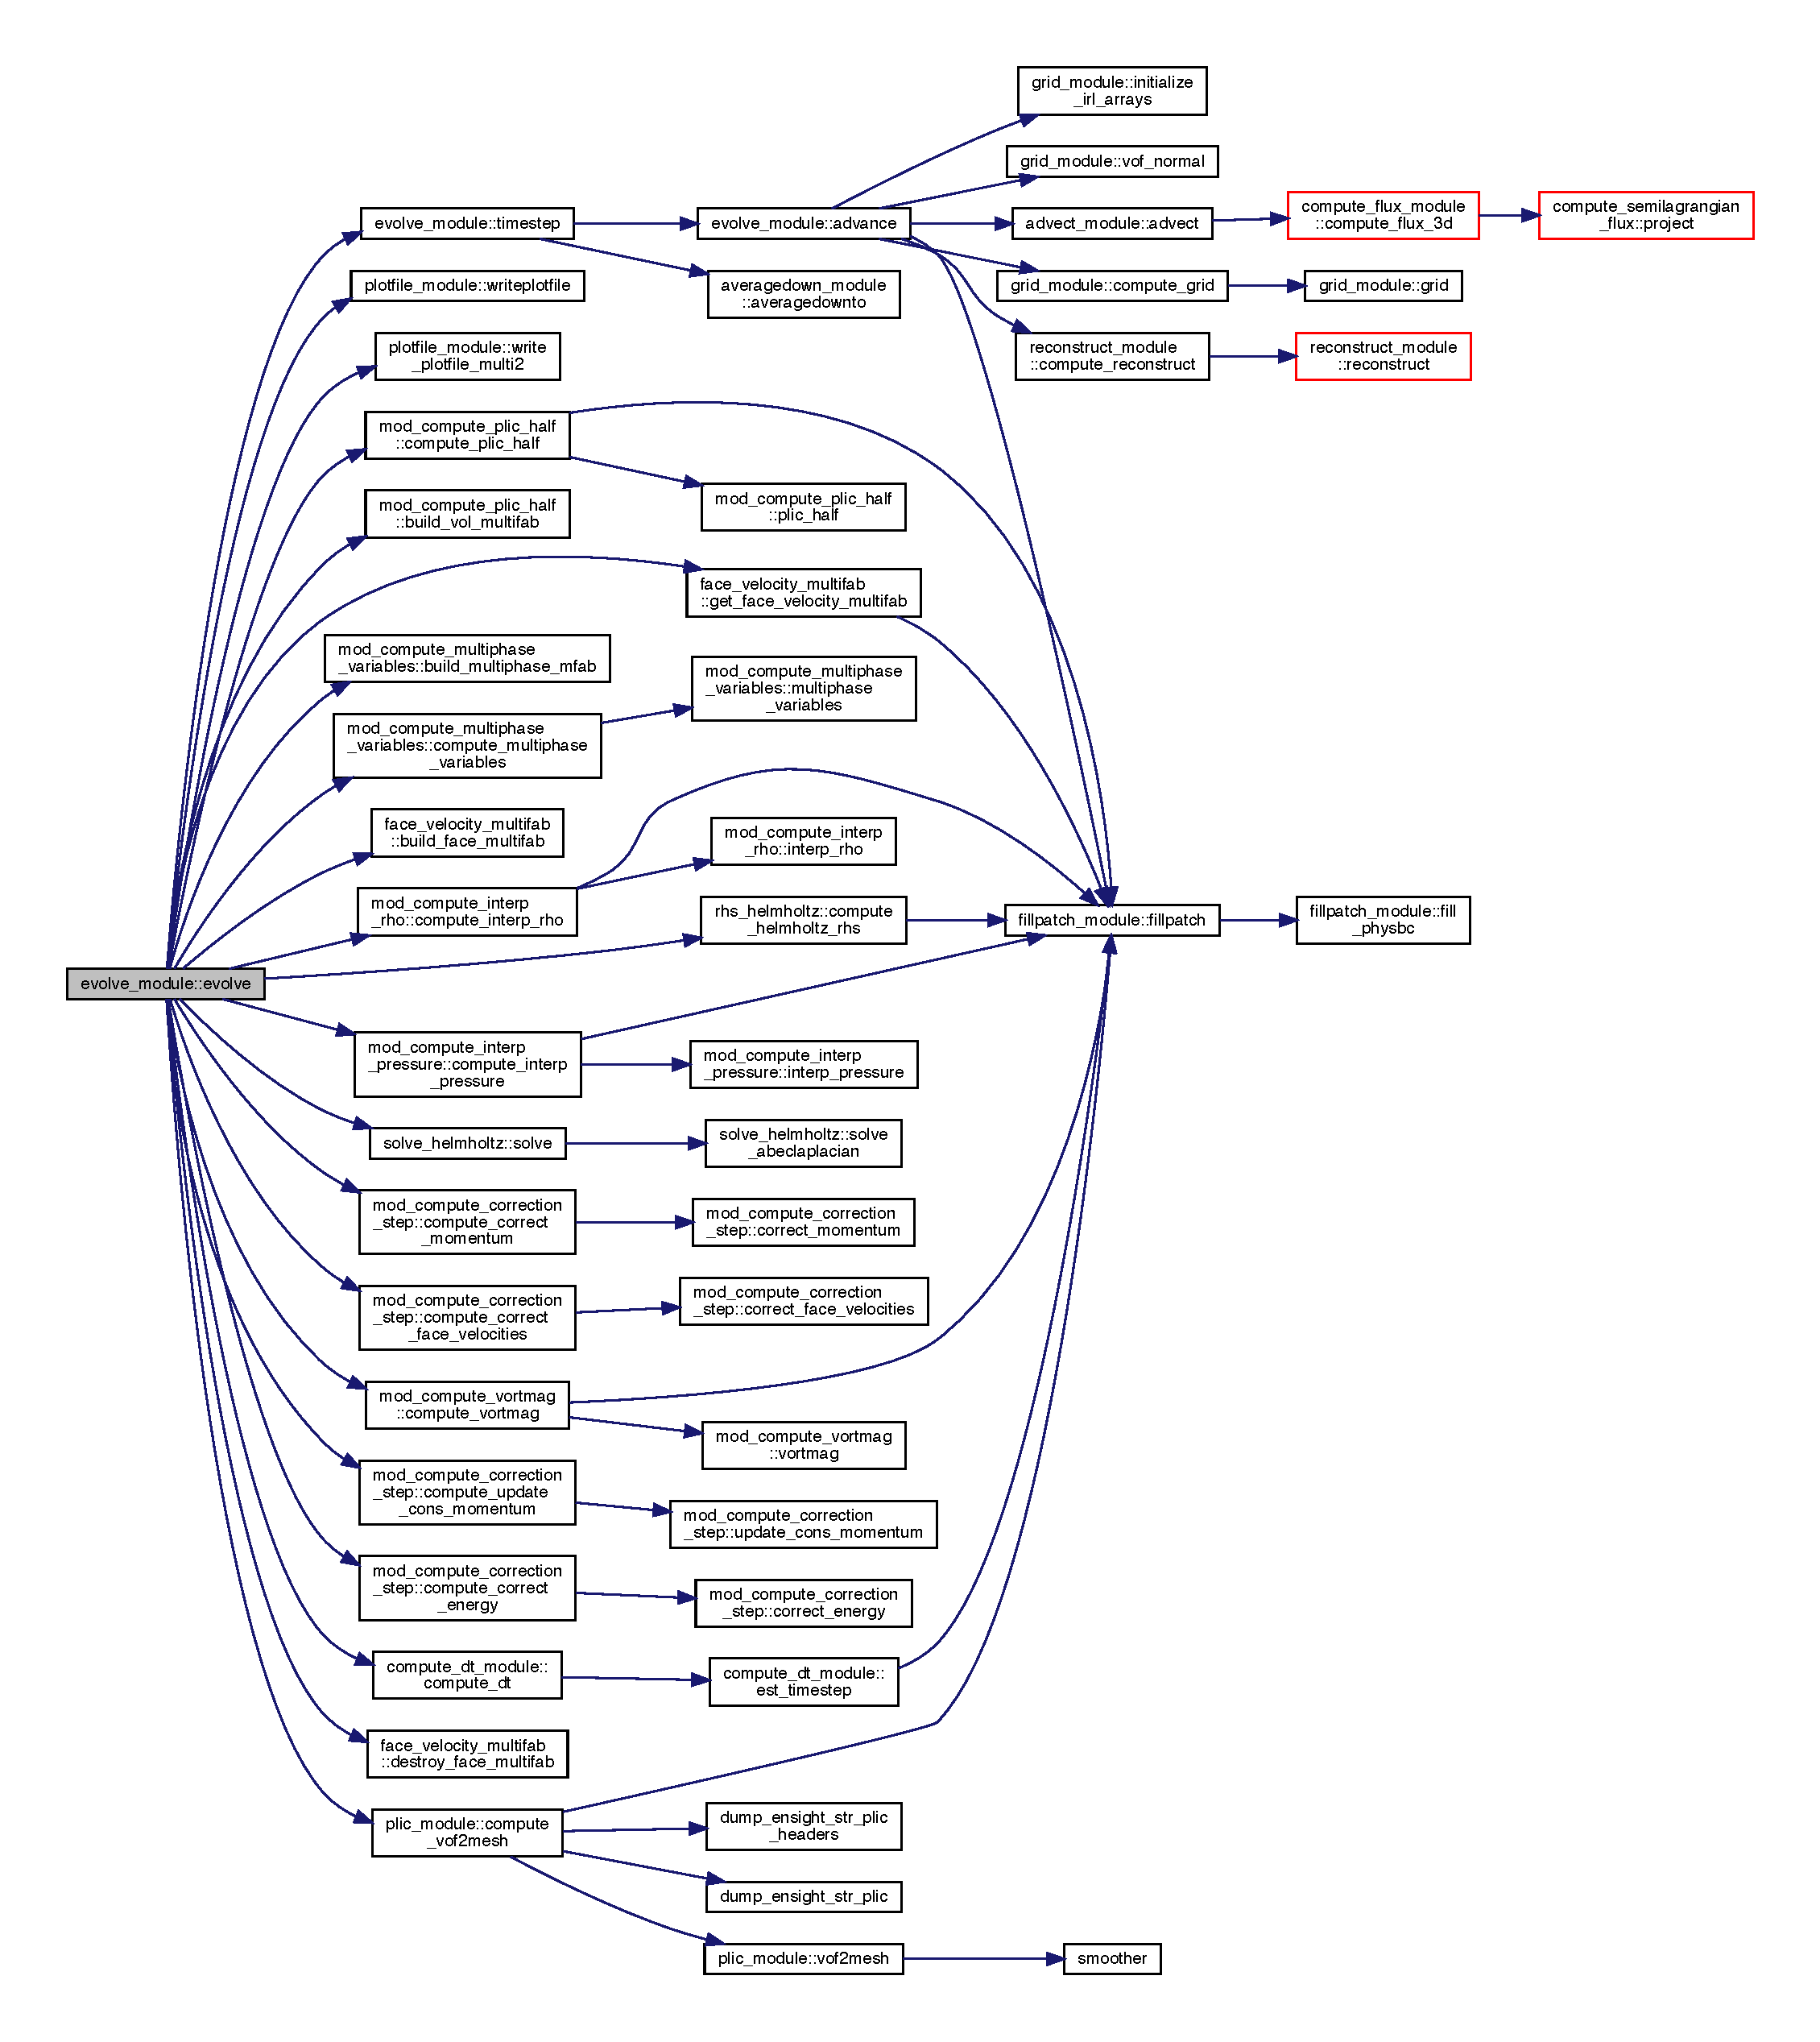
\includegraphics[scale=0.5]{evolve_mod_full.pdf}
\end{figure}

\begin{figure}
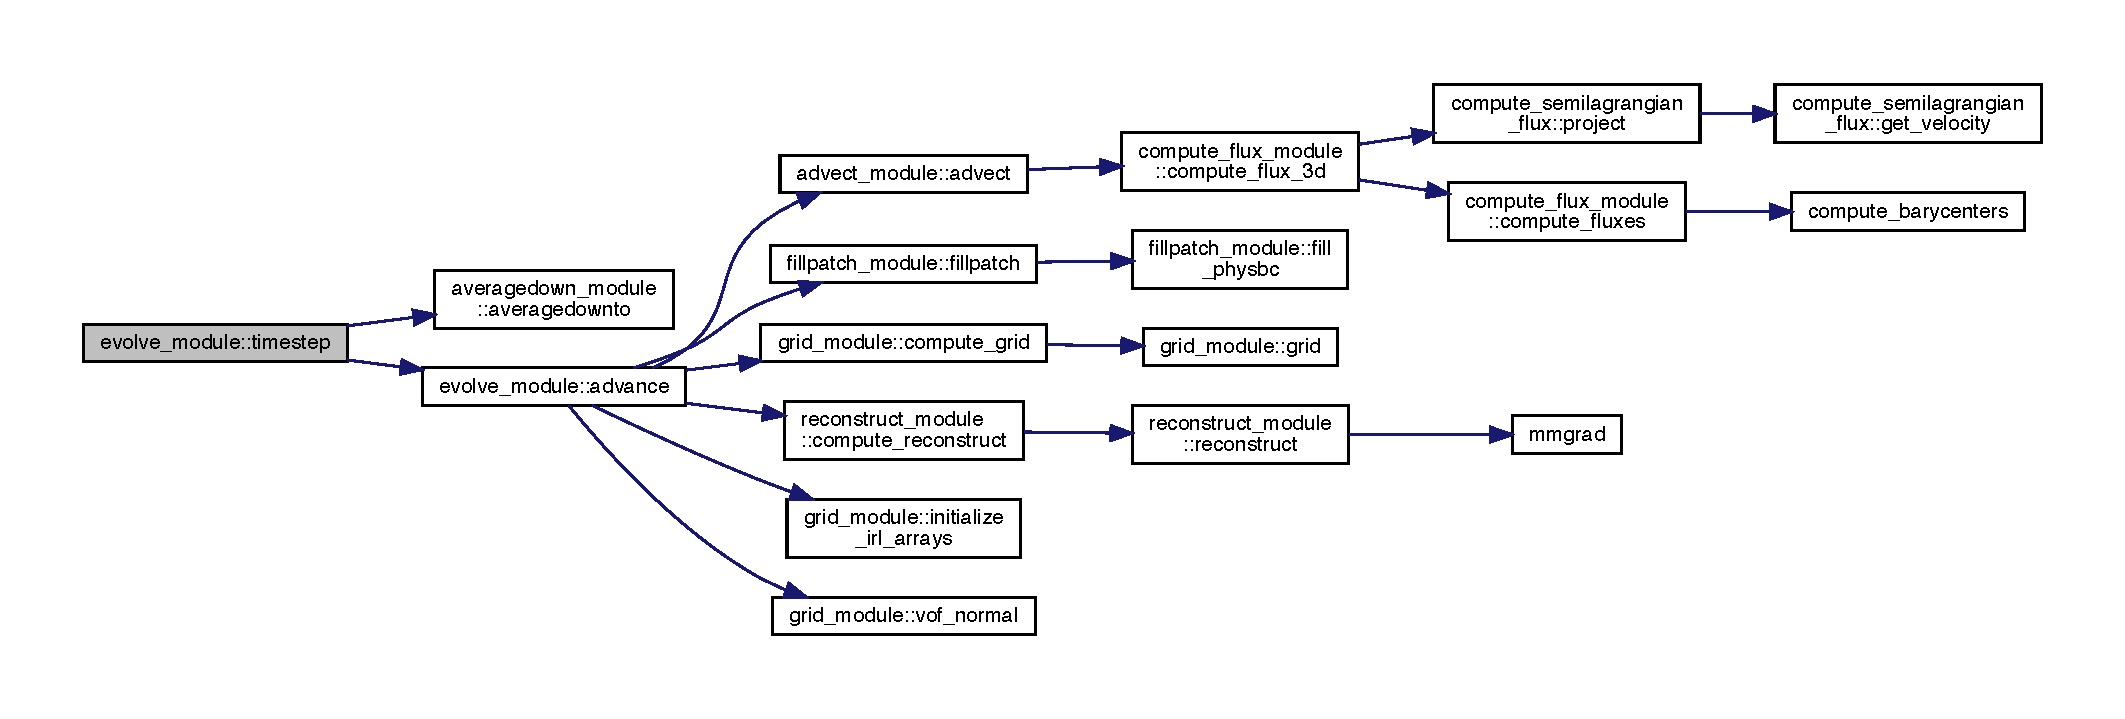
\includegraphics[scale=0.5]{evolve_mod_timestep.pdf}
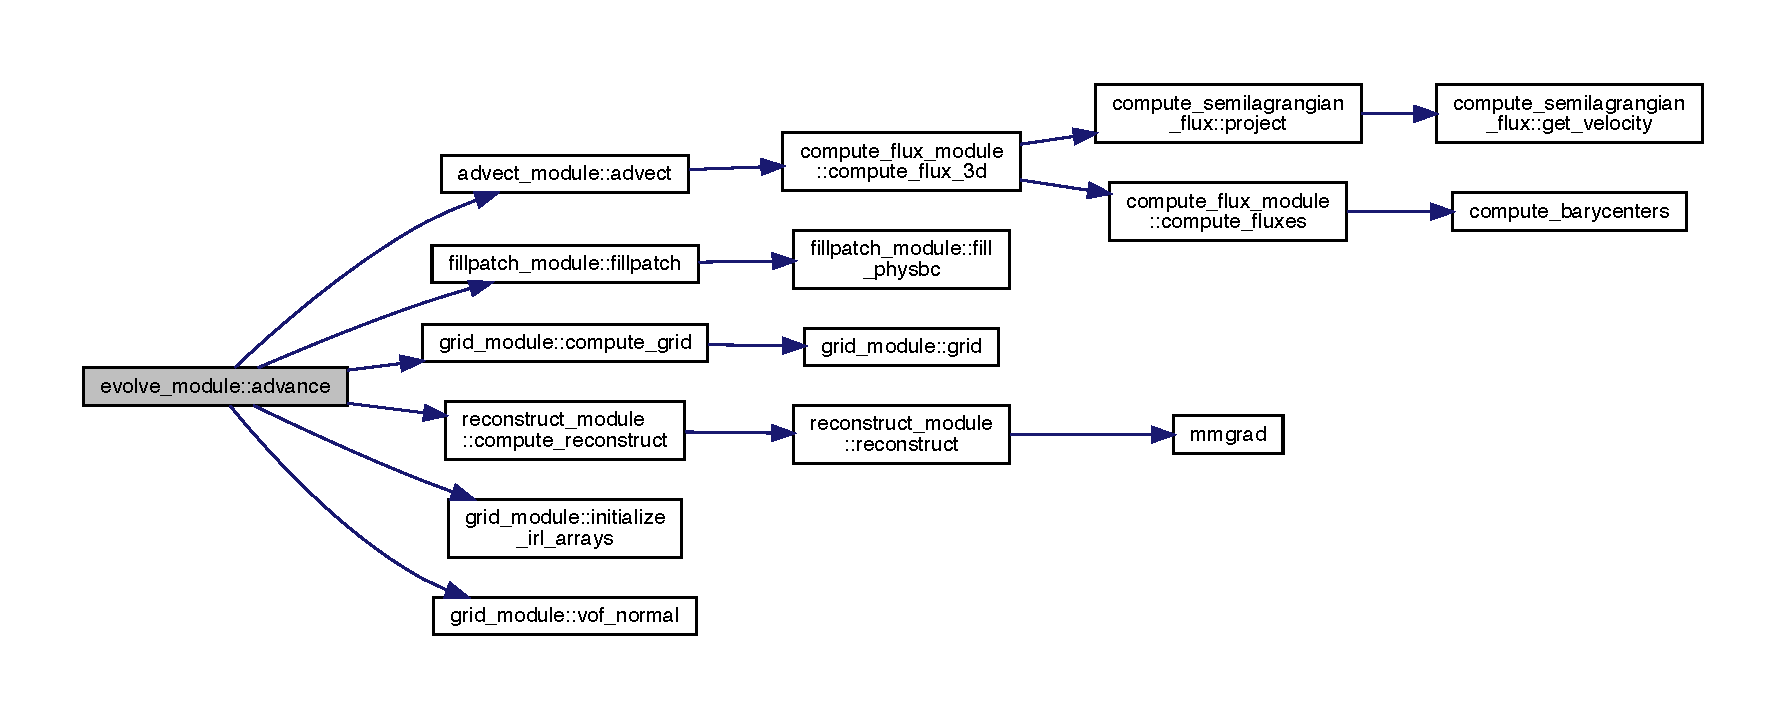
\includegraphics[scale=0.5]{evolve_mod_advance.pdf}
\end{figure}



\newpage	
\bibliographystyle{jfm}
\bibliography{Master}

\end{document}
